\section{May 2023}

\subsection*{Classical Mechanics}
\addcontentsline{toc}{subsection}{Classical Mechanics}

\prob{1.1}{

Write down the Lagrangian and the equation of motion for an ``old clock'' pendulum consisting of a weightless rod of length $l$ connected to a disk of radius $R$ and mass $M$ and moving in a gravitational field with normal acceleration $g$.
Calculate the period of small oscillations.
The moment of inertia of a disk relative to its center of mass is $I = M R^2 / 2$.

\begin{center}
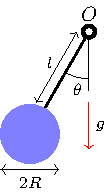
\includegraphics[scale=1.5]{May2023/1-1.pdf}
\end{center}

}

\sol{

The kinetic energy of an extended body calculated in the center of mass frame with an arbitrary origin is
\begin{align}
    T = \frac{M v^2}{2} + \frac{I \omega^2}{2}
.\end{align}
If we place our origin at the center of mass, then the velocity of the body is given as
\begin{align}
    v^2 = \dot{x}^2 + \dot{y}^2 = ( l + R )^2 \dot{\theta}^2
,\end{align}
and by construction $\omega = \dot{\theta}$.
Hence,
\begin{align}
    T = \frac{M (l + R)^2 \dot{\theta}^2}{2} + \frac{M R^2 \dot{\theta}^2}{4} = \frac{M [2(l+R)^2 + R^2] \dot{\theta}^2}{4}
.\end{align}
Note that we could also find this answer by placing our origin at the suspension point and using the parallel axis theorem.
In this frame, our origin coincides with the axis of rotation, so all of the kinetic energy is from rotation:
\begin{align}
    T = \frac{I' \omega^2}{2} = \Bigg[ \frac{MR^2}{2} + M (l + R)^2 \Bigg] \frac{\dot{\theta}^2}{2} = \frac{M [ 2(l + R)^2 + R^2 ] \dot{\theta}^2}{4}
\end{align}

The Lagrangian is then given as
\begin{align}
    \eqbox{ L = \frac{M [2(l + R)^2 + R^2] \dot{\theta}^2}{4} + mg (l + R) \cos{\theta} }
.\end{align}

The equation of motion is given by the Euler-Lagrange equation:
\begin{align}
    &\pdv{L}{\theta} - \dv{t} \pdv{L}{\dot{\theta}} = - Mg(l + R) \sin{\theta} - M \Big[ (l + R)^2 + \frac{R^2}{2} \Big] \ddot{\theta} = 0 \\
    &\Rightarrow \ddot{\theta} + \frac{2(l+R)^2 + R^2}{2g(l+R)} \sin{\theta} = 0
.\end{align}
From this we can see the angular frequency of small oscillations is given by
\begin{align}
    \eqbox{ \omega = \sqrt{\frac{g (l+R)}{(l + R)^2 + R^2/2}} \Rightarrow T = \frac{2 \pi}{\omega} = 2 \pi \sqrt{\frac{(l+R)^2 + R^2/2}{g(l+R)}} }
.\end{align}
Note that in the limit where $l \ll R$, the angular frequency approaches the simple pendulum result of $\omega = \sqrt{g/l}$.

}


\prob{1.2}{

A small asteroid of mass $m$ is moving from infinity with a velocity $v$ toward a planet of mass $M \gg m$ and radius $R$ as shown below.
Calculate the maximum impact parameter $b_{m}$ at which the asteroid with $b < b_m$ would crush onto the planet surface, assuming that the planet does not move.

\begin{center}
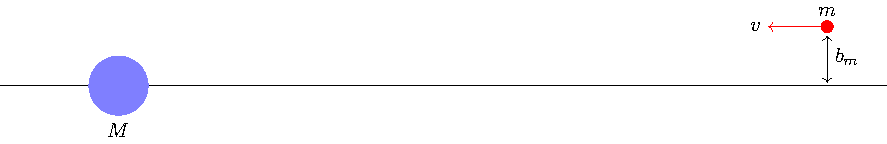
\includegraphics{May2023/1-2.pdf}
\end{center}

}

\sol{

Since the planet is much more massive than the asteroid, we can treat it as being fixed.
The condition for impact is that $r_{\rm min} < R$, where $U_{\rm eff}(r_{\rm min}) = E = m v^2 / 2 > 0$.
Our effective potential is given by
\begin{align}
    U_{\rm eff} = \frac{M^2}{2mr^2} - \frac{\alpha}{r}
,\end{align}
where the last term represents a generic attractive $1/r$ potential.
The angular momentum of the system is invariant and given by $M = m b v$.
Plugging this in, and setting the effective potential equal to the energy of the system, we have
\begin{gather}
    \frac{E b^2}{r_{\rm min}^2} - \frac{\alpha}{r_{\rm min}} = E \Rightarrow r_{\rm min} = \frac{2 E b^2}{\alpha + \sqrt{\alpha^2 + 4 E^2 b^2}} = \frac{m v^2 b^2/\alpha}{1 + \sqrt{1 + m^2 v^4 b^2 / \alpha^2}}
.\end{gather}
The maximum impact parameter at which impact occurs is such that
\begin{gather}
    r_{\rm min}(b_m) = R \nonumber \\
    R^2 + \frac{m^2 v^4 R^2}{\alpha^2} b_m^2 = \Big( \frac{mv^2}{\alpha} b_m^2 - R \Big)^2 = \Big( \frac{mv^2}{\alpha} \Big)^2 b_m^4 - \frac{2 m v^2 R}{\alpha} b_m^2 + R^2 \nonumber \\
    \eqbox{ b_m = \sqrt{ \frac{R \alpha}{m v^2} \Bigg[ 2 + \frac{m v^2 R}{\alpha} \Bigg] } = R \sqrt{ 1 + \frac{2 G M}{v^2 R} } }
,\end{gather}
where in the last equality we have inserted $\alpha = G M m$ for gravitational potentials.

}


\prob{1.3}{

A particle is constrained to move without friction along the surface of a sphere that is placed near the surface of the earth, where the gravitational field can be taken to be constant and uniform (see figure below).

\begin{parts}
    \item Write down the Lagrangian in spherical coordinates

    \item Derive the equations of motion.
\end{parts}

\begin{center}
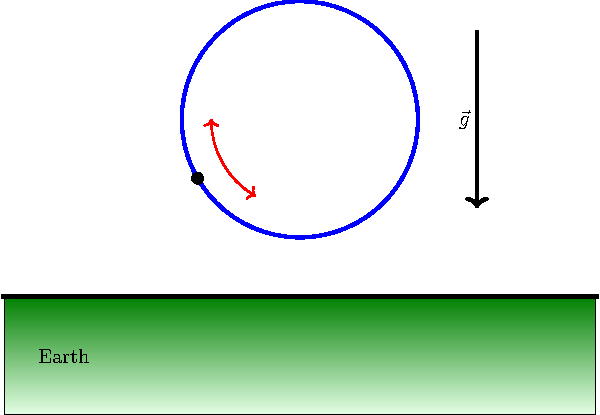
\includegraphics{May2023/1-3.pdf}
\end{center}

}

\sol{

(a) Let us call the radius of the sphere $R$.
The position of the particle can be parameterized as
\begin{align}
    \vec{r} = R [ \sin{\theta} \cos{\phi} \vhat{x} + \sin{\theta} \sin{\phi} \vhat{y} + \cos{\theta} \vhat{z} ]
,\end{align}
where we have placed our origin at the center of the sphere and the angles $\theta$ and $\phi$ are defined as usual.
The velocity is just the time derivative of this vector:
\begin{align}
    \vec{v} = R [ (\dot{\theta} \cos{\theta} \cos{\phi} - \dot{\phi} \sin{\theta} \sin{\phi}) \vhat{x} + (\dot{\theta} \cos{\theta} \sin{\phi} + \dot{\phi} \sin{\theta} \cos{\phi}) \vhat{y} - \dot{\theta} \sin{\theta} \vhat{z} ]
.\end{align}
Note that $R$ is constant in time.
Hence, the kinetic energy of the particle is given by
\begin{align}
    T = \frac{m R^2}{2} \Big[ \dot{\theta}^2 + \dot{\phi}^2 \sin^2{\theta} \Big]
,\end{align}
where $m$ is the mass of the particle.
Next, we write down the potential energy of the particle, setting our reference point at the origin:
\begin{align}
    U = m g z = m g R \cos{\theta}
.\end{align}
Putting these together, the Lagrangian reads
\begin{align}
    \eqbox{ L = \frac{m R^2}{2} \Big[ \dot{\theta}^2 + \dot{\phi}^2 \sin^2{\theta} \Big] - m g R \cos{\theta} }
\end{align}


(b) From the Lagrangian, the equations of motion are
\begin{align}
\eqbox{
\begin{aligned}
    m R^2 \ddot{\theta} + m g R \sin{\theta} - m R^2 \dot{\phi}^2 \sin{\theta} \cos{\theta} &= 0 \\
    m R^2 \ddot{\phi} \sin^2{\theta} &= 0
.\end{aligned}
}
\end{align}
Notice that the second equation is really just a conservation equation.
That is, $\phi$ is a cyclic coordinate, meaning that its conjugate momentum
\begin{align}
    p_{\phi} = m R^2 \dot{\phi} \sin^2{\theta}
\end{align}
is a constant of motion.
We can use this to rewrite our first equation of motion as
\begin{align}
    \ddot{\theta} + \frac{g}{R} \sin{\theta} - \frac{p_{\phi}^2}{m R^2 \sin^{3}{\theta}\tan{\theta}} = 0
.\end{align}
From this, one recognizes the simple pendulum terms on the left and a last term from the rotating plane of oscillation.

}


\prob{1.4}{

Physicists sometimes use the Lennard-Jones 6-12 potential
\begin{align*}
    V(r) = \frac{A}{r^{12}} - \frac{B}{r^6}
\end{align*}
to describe the interaction between the atoms in a diatomic molecule, where $A$ and $B$ are constant parameters.
Let the atoms in the molecule have masses $m_A$ and $m_B$, respectively.
For small departures from the equilibrium separation $r_0$, find the angular frequency of oscillations for the diatomic system in terms of $A$, $B$, and the masses.
For this problem, you may assume that the methods of classical mechanics apply, and that quantum mechanical effects are negligible.

}

\sol{

The energy of the system
\begin{align}
    E = \frac{\mu \dot{r}^2}{2} + \frac{M^2}{2 \mu r^2} + \frac{A}{r^{12}} - \frac{B}{r^6}
,\end{align}
where $\mu = m_A m_B / (m_A + m_B)$ is the reduced mass of the system and $M$ is the angular momentum of the system.
The last three terms are the effective potential of the system, that is
\begin{align}
    U_{\rm eff}(r) = \frac{M^2}{2 \mu r^2} + \frac{A}{r^{12}} - \frac{B}{r^6}
.\end{align}
First, we define the equilibrium separation $r_0$ such that $U_{\rm eff}'(r_0) = 0$.
For small departures from this equilibrium, we can write
\begin{align}
    U_{\rm eff}(r) &= U_{\rm eff}(r_0) + U_{\rm eff}'(r_0) (r - r_0) + \frac{U_{\rm eff}''(r_0)}{2!} (r - r_0)^2 + ... \nonumber \\
    &\approx U_{\rm eff}(r_0) + \frac{U_{\rm eff}''(r_0)}{2!} (r - r_0)^2
.\end{align}
The equation of motion for such a system is then
\begin{align}
    m \Delta \ddot{r} + U_{\rm eff}''(r_0) \Delta r = 0
,\end{align}
where $\Delta r = r - r_0$ obeys the simple harmonic oscillator equation with angular frequency $\omega = \sqrt{U_{\rm eff}''(r_0) / m}$.
Notice the difficulty, though, in solving this problem, in generality, analytically:
\begin{align}
    U_{\rm eff}'(r_0) &= -\frac{M^2}{\mu r_0^3} - \frac{12 A}{r_0^{13}} + \frac{6 B}{r_0^7} = 0 \\
    U_{\rm eff}''(r_0) &= \frac{3 M^2}{\mu r_0^4} + \frac{12(13) A}{r_0^{14}} - \frac{6(7) B}{r_0^8}
.\end{align}
Solving the former of these for the equilibrium separation requires solving for the roots of a $10^{\rm th}$ order polynomial, which has no known closed form solution.

For now, we will simplify our lives and assume that $M = 0$.
In this case $U_{\rm eff}(r) = V(r)$, and the equilibrium point $r_0$ is just
\begin{align}
    r_0 = \Big( \frac{2 A}{B} \Big)^{1/6}
.\end{align}
The second derivative of the potential at this point is then
\begin{align}
    U_{\rm eff}''(r_0) &= 6 \Big( \frac{B}{2A} \Big)^{1/3} \Bigg[ 26 A \Big( \frac{B^2}{4 A^2} \Big) -  7 B \Big( \frac{B}{2 A} \Big) \Bigg] = \frac{18 B^2}{A} \Big( \frac{B}{2 A} \Big)^{1/3} 
,\end{align}
and the frequency of small oscillations reads
\begin{align}
    \eqbox{ \omega = 3 B \sqrt{\frac{2}{m A} \Big( \frac{B}{2A} \Big)^{1/3}} }
\end{align}

}


\prob{2.1}{

A round hole is cut off a homogeneous disk of radius $R$ as shown in the Figure.
The mass of the remaining part (it is solid in the figure) equals $m$.
Find the moment of inertia of such a disk with respect to an axis perpendicular to the disk surface and going through:

\begin{parts}
    \item the point $O$ (see Figure);

    \item its center of mass.
\end{parts}

\begin{center}
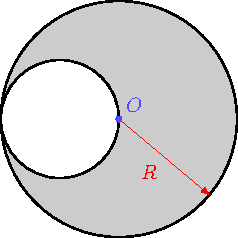
\includegraphics{May2023/2-1.pdf}
\end{center}

}

\sol{

(a) Observe that the elements of the moment of inertia tensor are given by
\begin{align}
    I_{ij} = \int \dd[3]{\vec{r}} (r^2 \delta_{ij} - x_i x_j) \rho(\vec{r})
.\end{align}
Since this is linear in the mass density, we can construct the hole by summing the moments of inertia from a full disk (no hole) centered at $O$ with density $\rho = m/[\pi(R^2 - (R/2)^2)] = 4 m / (3 \pi R^2)$ (i.e. total mass $m_1 = \rho \pi R^2 = 4m/3$) and a smaller disk (offset by $R/2$ to the left of $O$) with mass density $-\rho$ (i.e. total mass $m_2 = -\rho \pi (R/2)^2 = -m/3$).
That is,
\begin{align}
    \eqbox{ I = \frac{1}{2} m_1 R^2 + \Bigg[ \frac{1}{2} m_2 \Big( \frac{R}{2} \Big)^2  + m_2 \Big( \frac{R}{2} \Big)^2 \Bigg] = \frac{13}{24} m R^2 }
,\end{align}
where we have use that for a disk with mass $M$ and radius $r$, the moment of inertia about an axis perpendicular to its face is $I_{\rm disk} = M r^2 / 2$.


(b) Observe that the center of mass of any body
\begin{align}
    \vec{R} = \frac{1}{M} \int \dd[3]{\vec{r}} \vec{r} \rho(\vec{r})
,\end{align}
so for our body, we can use the same trick as above:
\begin{align}
    R = \frac{m_1 R_1 + m_2 R_2}{m} =  -\frac{m_2}{m} \frac{R}{2} = \frac{R}{6}
.\end{align}
Hence, using the parallel axis theorem and the result above, the moment of inertia of the disk above about its center of mass is
\begin{align}
    \eqbox{ I_{\rm CM} = \frac{13}{24} m R^2 - m \Big( \frac{R}{6} \Big)^2 = \frac{37}{72} m R^2 }
.\end{align}

}

\subsection*{Electricity \& Magnetism}
\addcontentsline{toc}{subsection}{Electricity \& Magnetism}

\prob{2.2}{

A charged sphere of radius $a$ and centered at $O$ has a spherically symmetric charge density $\rho(r)$ that varies radially as $\rho(r) = \alpha r^2$.
The total charge of the sphere is $Q$.

This charged sphere is surrounded by a grounded conducting sphere of radius $b > a$ that is also centered at $O$ (see Figure).

\begin{parts}
    \item Find electric field $\bf{E}(\bf{r})$ everywhere in space.

    \item Find the electrostatic potential $\Phi(\bf{r})$ everywhere in space.
\end{parts}

\begin{center}
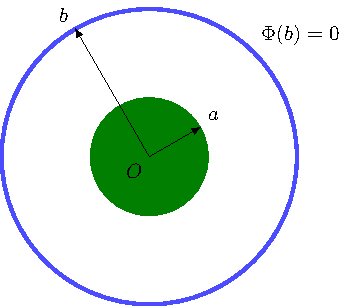
\includegraphics{May2023/2-2.pdf}
\end{center}

}

\sol{

(a) We can determine the electric field easily from Gauss' law
\begin{align}
    \oint_S \vb*{E} \cdot \dd{\vb*{S}} = \frac{q}{\epsilon_0}
,\end{align}
which is only practically useful when we have some kine of symmetry -- in this case, radial.
Note that $q$ is the charge enclosed by the surface $S$.
For this problem, the electric field must be radial, so we choose spherical surfaces:
\begin{align}
    E_r (4 \pi r^2) = \frac{4 \pi \alpha}{\epsilon_0} \int \dd{r'} r'^4 \Theta(r \leq a) = \frac{4 \pi \alpha}{5 \epsilon_0} r_{<}^5
,\end{align}
where $r_{<} = \min(r,a)$.
Note that this result only holds for $r < b$.
The presence of the conducting sphere at $r = b$ shields the space external to this conductor from the electric field.
That is, for $r \geq b$, $\vb*{E} = 0$.
As a last step, we should exchange $\alpha$ for $Q$ by normalizing the charge density as follows:
\begin{align}
    Q = 4\pi \alpha \int_{0}^{a} \dd{r} r^4 = \frac{4 \pi a^5}{5} \alpha
.\end{align}
Thus, for $r < b$, we have
\begin{align}
    E_r = \frac{Q}{4 \pi \epsilon_0 a^2} \frac{r_<^5}{a^3 r^2} = \frac{Q}{4 \pi \epsilon_0 a^2} \begin{cases}
        (r/a)^3 & r < a \\
        (a/r)^2 & a < r < b
    .\end{cases}
\end{align}

(b) Using the electric field, we can determine the potential by using
\begin{align}
    \Phi(\vb*{r}) = -\int_{\vb*{r}_0}^{\vb*{r}} \vb*{E} \cdot \dd{\vb*{r}}
.\end{align}
Note that for $r \geq b$, our potential $\Phi = 0$ since the electric field is zero in this region and the sphere is grounded.
Inside the sphere, with $r > a$, we have
\begin{align}
    \Phi(a < r < b) = \frac{Q}{4 \pi \epsilon_0} \int_{r}^{b} \frac{\dd{r}}{r^2} = \frac{Q}{4 \pi \epsilon_0 b} \Big( \frac{b}{r} - 1 \Big)
,\end{align}
and for $r < a$, we have
\begin{align}
    \Phi(r < a) &= \frac{Q}{4 \pi \epsilon_0} \Bigg[ \Big( \frac{1}{a} - \frac{1}{b} \Big) + \frac{1}{a^5} \int_{r}^{a} r^3 \dd{r} \Bigg] \nonumber \\
    &= \frac{Q}{4 \pi \epsilon_0} \Bigg[ \frac{1}{a} - \frac{1}{b} + \frac{a^4 - r^4}{4a^5} \Bigg] \nonumber \\
    &= \eqbox{ \frac{Q}{4 \pi \epsilon_0 a} \Bigg[ \frac{5}{4} - \frac{a}{b} - \frac{1}{4} \Big( \frac{r}{a} \Big)^4 \Bigg] }
\end{align}

}


\prob{2.3}{

Two metal objects of arbitrary shape are embedded in a conducting material of uniform conductivity $\sigma$.

\begin{parts}
    \item Derive a relationship between the resistance, $R$, between the objects and the mutual capacitance, $C$.

    \item The two objects are charged to a potential difference $V_0$.
    If the battery is then disconnected, derive an expression for the potential difference as a function of time in terms of $\sigma$ and $\epsilon_0$.
\end{parts}

}

\sol{

(a) Ohm's law reads $\vec{J} = \sigma \vec{E}$.
If we integrate over a Gaussian surface enclosing one of the spheres, which has charge $Q$, we find
\begin{align}
    I = \int \vec{J} \cdot \dd{\vec{A}} = \sigma \int \vec{E} \dd{\vec{A}} = \frac{\sigma Q}{\epsilon_0}
.\end{align}
Next, we use the definition of capacitance to write
\begin{align}
    C = \frac{Q}{V} \Rightarrow V = I \Big( \frac{\epsilon_0}{\sigma C} \Big)
.\end{align}
That is, the resistance
\begin{align}
    \eqbox{ R = \frac{\epsilon_0}{\sigma C} }
\end{align}

(b) The current between the spheres
\begin{align}
    I = -\dv{Q}{t} = \frac{V}{R} = \frac{Q}{RC} \Rightarrow Q(t) = Q_0 e^{- (\sigma / \epsilon_0) t} \Rightarrow \eqbox{ V(t) = V_0 e^{-(\sigma/\epsilon_0) t} }
.\end{align}

}


\prob{2.4}{

A relativistic positively charged particle of charge $q$ and mass $m$ is traveling with velocity $v_0$ in the negative $z$-direction as shown in the figure.
At $z=0$, the particle enters a semi-infinite region $z < 0$ of homogeneous electric field directed in the positive $z$ direction $\vb*{E} = E \hat{z}$.
How far does the particle penetrate into the $z < 0$ region and how much time does is spend there?
Neglect the Abraham-Lorentz force of radiation reaction.

\begin{center}
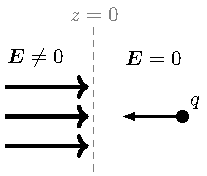
\includegraphics{May2023/2-4.pdf}
\end{center}

}

\sol{

Ignoring, the Abraham-Lorentz force of radiation, we simply have
\begin{align}
    \dv{\vb*{p}}{t} = q \vb*{E}
,\end{align}
where $p$ is the relativistic three-momentum of the particle.
Since the motion is entirely constrained to the $z$-axis, we have
\begin{align}
    \dv{p_z}{t} = q E \Rightarrow p_z = p_0 + q E t
,\end{align}
where
\begin{align}
    p_0 = - \gamma_0 m v_0 = -\frac{mv_0}{\sqrt{1 - v_0^2/c^2}}
\end{align}
Next, we determine the velocity of the particle as a function of time through
\begin{align}
    \vb*{p} = \gamma m \vb*{v} = \frac{\mathcal{E}}{mc^2} m \vb*{v} = \frac{\mathcal{E}}{c^2} \vb*{v}
,\end{align}
where $\mathcal{E} = c \sqrt{(mc)^2 + \vb*{p}^2}$ is the relativistic energy of the particle, so
\begin{align}
    v = \frac{c^2}{\mathcal{E}} [qEt + p_0] = c \frac{q E c t - |p_0| c}{\sqrt{(mc^2)^2 + (q E c t - |p_0| c)^2}}
.\end{align}
This is related to the position as follows:
\begin{align}
    z = c \int_0^t \dd{t'} \frac{q E c t' - |p_0|c}{\sqrt{(mc^2)^2 + (q E c t' - |p_0|c)^2}}
.\end{align}
The above integral can be solved by utilizing the substitution
\begin{align}
    q E c t' - |p_0| c = mc^2  \sinh{u} \Rightarrow q E c \dd{t'} = mc^2 \cosh{u} \dd{u}
\end{align}
such that
\begin{align}
    z &= c \int_{u(0)}^{u(t)} \dd{u} \frac{mc^2}{q E c} \cosh{u} \frac{mc^2 \sinh{u}}{mc^2 \cosh{u}} = \frac{mc^2}{q E} \int_{u(0)}^{u(t)} \dd{u} \sinh{u} \nonumber \\
    &= \frac{mc^2}{q E} [\cosh{u(t)} - \cosh{u(0)}] \nonumber \\
    &= \frac{1}{q E} \Big[ \sqrt{(mc^2)^2 + (q E c t - |p_0|c)^2} - \sqrt{(mc^2)^2 + (|p_0|c)^2} \Big]
,\end{align}
where we have used the fact that $\cosh^2{x} = 1 + \sinh^2{x}$.

We now have all the information needed to determine the time the particle spends in the region $z < 0$ and how far the particle penetrates within this region.
The penetration distance is determined by the turning point, where
\begin{align}
    p = 0 \Rightarrow T = -\frac{p_0}{qE} = \frac{|p_0|}{qE}
\end{align}
so that
\begin{align}
    \eqbox{ |z(T)| = \frac{mc^2}{qE} \Big| \sqrt{1 + \Big( \frac{|p_0|c}{mc^2} \Big)^2 } - 1 \Big| }
.\end{align}
Next, the time the particle spends in the negative-$z$ region is defined by the equation
\begin{align}
    z(t) = 0 \Rightarrow \eqbox{ t = \frac{|p_0| c \pm |p_0| c}{q E c} = \frac{2 |p_0|}{q E} = 2 T }
,\end{align}
where we take the $+$ branch since the $-$ branch gives the entry time of the particle into the $z < 0$ region.
Classically, it is obvious to us that the total time in this region is twice the time before the turning point since the position is quadratic in time, symmetric with respect to the turning point.
Relativistically, though, it may not be so obvious since the dependence of the velocity and position on time is more complicated.
Still, however, the total time is double the time to the turning point, and fundamentally, this is because of time-reversal symmetry.
That is, the motion of the particle out of the $z > 0$ region is just the braking portion of the particle's motion in reverse.

}


\prob{3.1}{

A thin circular ring of radius $R$ lies in the $xy$-plane and is centered at the origin.
It consists of two semicircles (corresponding to $y > 0$ and $y < 0$) that are uniformly charged with opposite charges $+q$ and $-q$.

Determine the electrostatic potential $\Phi$ and electric field $\vb*{E}$ on the $z$ axis (it goes through the center of the ring) and near that axis.

What is the asymptotic behavior of the field at very large distances from the ring?

\begin{center}
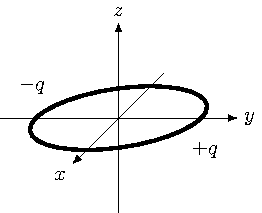
\includegraphics{May2023/3-1.pdf}
\end{center}

}

\sol{

We can determine the potential via
\begin{align}
    \Phi(\vb*{r}) = \frac{1}{4 \pi \epsilon_0} \int \dd[3]{\vb*{r}'} \frac{\rho(\vb*{r}')}{|\vb*{r} - \vb*{r}'|}
.\end{align}
The charge density is simply given as
\begin{align}
    \rho(\vb*{r}) = \frac{q}{\pi R^2} \delta(r - R) \delta(\cos{\theta}) \Big[ \Theta(0 \leq \phi \leq \pi) - \Theta(\pi \leq \phi \leq 2 \pi) \Big]
.\end{align}
One can verify that this in fact gives the required total charge $q$ for the $y > 0$ portion of the ring and $-q$ for the $y < 0$ portion of the ring.
Thus, we have
\begin{align}
    \Phi(\vb*{r}) = \frac{q}{4 \pi \epsilon_0} \frac{1}{\pi} \int_{0}^{2 \pi} \frac{\Theta(0 \leq \phi' \leq \pi) - \Theta(\pi \leq \phi'  \leq 2 \pi)}{\sqrt{ r^2 + R^2 - 2 \vb*{r} \cdot \vb*{r}' }} \dd{\phi'}
.\end{align}
Since we care first to evaluate the potential for points on the $z$ axis, we take $\vb*{r} = z \vu*{z}$, yielding
\begin{align}
    \Phi(\vb*{r}) &= \frac{q}{4 \pi \epsilon_0} \frac{1}{\pi} \int_{0}^{2 \pi} \frac{\Theta(0 \leq \phi' \leq \pi) - \Theta(\pi \leq \phi' \leq 2 \pi)}{\sqrt{z^2 + R^2}} \dd{\phi'} = 0
.\end{align}
To go off the $z$-axis, we write
\begin{align}
    \vec{r} \cdot \vec{r}' &= r r' [ \sin{\theta} \sin{\theta'} \cos(\phi - \phi') + \cos{\theta} \cos{\theta'} ] \nonumber \\
    &= r R \sin{\theta} \cos(\phi - \phi')
,\end{align}
where in the last equality, we have enforced the $\delta$ functions for the charge density.
We insert this into the generic expression for the potential and find
\begin{align}
    \Phi(\vec{r}) &= \frac{q}{4 \pi \epsilon_0} \frac{1}{\pi} \int_{0}^{2 \pi} \frac{\Theta(0 \leq \phi' \leq \pi) - \Theta(\pi \leq \phi' \leq 2 \pi)}{\sqrt{r^2 + R^2 - 2 r R \sin{\theta} \cos(\phi - \phi')}} \nonumber \\
    &= \frac{q}{4 \pi \epsilon_0} \frac{1}{\pi} \int_{0}^{\pi} \dd{\phi'} \Bigg[ \frac{1}{\sqrt{r^2 + R^2 - 2 r R \sin{\theta} \cos(\phi - \phi')}} - \frac{1}{\sqrt{r^2 + R^2 + 2 r R \sin{\theta} \cos(\phi - \phi')}} \Bigg]
\end{align}
We next want to find the potential just slightly off the $z$-axis, which implies that $r \sin{\theta} \ll R$ such that
\begin{align}
    \Big[ r^2 + &R^2 \pm 2 r R \sin{\theta} \cos(\phi - \phi') \Big]^{-1/2} = \frac{1}{\sqrt{r^2 + R^2}} \Bigg[ 1 \pm \frac{2R r \sin{\theta} \cos(\phi - \phi')}{r^2 + R^2} \Bigg]^{-1/2} \nonumber \\
    &= \frac{1}{\sqrt{r^2 + R^2}} \Bigg[ 1 \mp \frac{R r \sin{\theta}}{r^2 + R^2} \cos(\phi - \phi') + \hdots \Bigg]
.\end{align}
Inserting this expansion, the potential takes the form
\begin{align}
    \Phi(\vec{r}) &= \frac{q}{4 \pi \epsilon_0} \frac{1}{\pi \sqrt{r^2 + R^2}} \int_0^{\pi} \dd{\phi'} \Bigg[ \frac{2 R r \sin{\theta}}{r^2 + R^2} \cos(\phi - \phi') + ... \Bigg] \nonumber \\
    &\approx \frac{q}{4 \pi \epsilon_0} \frac{4 R r \sin{\theta} \sin{\phi}}{\pi (r^2 + R^2)^{3/2}}
.\end{align}
This also gives us the previous result on the $z$-axis since $\sin{\theta} = 0$ there.
Finally, let's determine the form of the potential when $r \gg R$ such that
\begin{align}
    \Big[ r^2 + &R^2 \pm 2 R r \sin{\theta} \cos(\phi - \phi') \Big]^{-1/2} = \frac{1}{r} \Bigg[ 1 \pm \frac{2 R \sin{\theta} \cos(\phi - \phi')}{r} + \frac{R^2}{r^2} \Bigg]^{-1/2} \nonumber \\
    &= \frac{1}{r} \Bigg[ 1 \mp \frac{R \sin{\theta} \cos(\phi - \phi')}{r} + \hdots \Bigg]
.\end{align}
Thus, the potential
\begin{align}
    \Phi(\vec{r}) \approx \frac{q}{4 \pi \epsilon_0} \frac{4 R \sin{\theta} \sin{\phi}}{\pi r^2}
.\end{align}
This is just a dipole potential.
Let's place our charges $+q$ at $y = d/2$ and $-q$ at $y = -d/2$.
The dipole moment is then just $\vec{p} = q d \vhat{y}$, and the potential
\begin{align}
    \Phi(\vec{r}) &= \frac{q}{4 \pi \epsilon_0} \Bigg[ \frac{1}{|\vec{r} - \vec{r}_+|} - \frac{1}{|\vec{r} - \vec{r}_-|} \Bigg] \nonumber \\
    &= \frac{q}{4 \pi \epsilon_0} \Bigg[ \frac{1}{\sqrt{r^2 + d^2/4 - 2 \vec{r} \cdot \vec{r}_+}} - \frac{1}{\sqrt{r^2 + d^2/4 - 2 \vec{r} \cdot \vec{r}_-}} \Bigg] \nonumber \\
    &\approx \frac{\vhat{n} \cdot \vec{p}}{4 \pi \epsilon_0 \, r^2} = \frac{q d \sin{\theta} \sin{\phi}}{4 \pi \epsilon_0 \, r^2}
.\end{align}
Next, we determine $d$ by integrating over the position vector, weighted by the charge distribution:
\begin{align}
    \vec{p} &= \int \dd[3]{\vec{r}} \vec{r} \rho(\vec{r}) = \frac{q R}{\pi} \int_{0}^{2 \pi} [ \cos{\phi} \vhat{x} + \sin{\phi} \vhat{y} ] [ \Theta(0 \leq \phi \leq \pi) - \Theta(\pi \leq \phi \leq 2\pi) ] \nonumber \\
    &= q \frac{4 R}{\pi} \vhat{y} \Rightarrow \Phi(\vec{r}) = \frac{q}{4 \pi \epsilon_0} \frac{4 q R \sin{\theta} \sin{\phi}}{\pi r^2}
.\end{align}
We thus see that our work is all self-consistent.

% For the electric field, we can take the gradient of the potential:
% \begin{align}
%     \vec{E} &= -\grad \Phi = - \pdv{\Phi}{r} \vhat{r} - \frac{1}{r} \pdv{\Phi}{\theta} \vhat{\theta} - \frac{1}{r\sin{\theta}} \pdv{\Phi}{\phi} \vhat{\phi} \nonumber \\
%     &= -\frac{q}{4 \pi \epsilon_0} \frac{4R}{\pi} \Bigg[ \sin{\theta} \sin{\phi} \pdv{r} \Big( \frac{r}{(r^2 + R^2)^{3/2}} \Big) \vhat{r} + \frac{\cos{\theta} \sin{\phi}}{(r^2 + R^2)^{3/2}} \vhat{\theta} + \frac{\cos{\phi}}{(r^2 + R^2)^{3/2}} \vhat{\phi} \Bigg] \nonumber \\
%     &= \eqbox{ -\frac{q}{4 \pi \epsilon_0} \frac{4R}{\pi} \Bigg[ \frac{(r^2 + R^2)^{3/2} - 3 r^3 \sqrt{r^2 + R^2}}{(r^2 + R^2)^{3}} \sin{\theta} \sin{\phi} \vhat{r} + \frac{\cos{\theta} \sin{\phi}}{(r^2 + R^2)^{3/2}} \vhat{\theta} + \frac{\cos{\phi}}{(r^2 + R^2)^{3/2}} \vhat{\phi} \Bigg] }
% .\end{align}
% On the $z$-axis, we have to do a bit more work.
% Recall that
% \begin{align}
%     \vhat{\theta} &= \cos{\theta} \cos{\phi} \vhat{x} + \cos{\theta} \sin{\phi} \vhat{y} - \sin{\theta} \vhat{z} \\
%     \vhat{\phi} = -\sin{\phi} \vhat{x} + \cos{\phi} \vhat{y}
% .\end{align}
% \begin{align}
%     \vec{E} = \frac{q}{4 \pi \epsilon_0} \frac{1}{\pi} \int_{0}^{2 \pi}
% \end{align}

}


\prob{3.2}{

Helmholtz coils are sometimes used by physicists to determine the charge to mass ratio of the electron.
From Wikipedia:

``A Helmholtz coil is a device for producing a region of nearly uniform
magnetic field, named after the German physicist Hermann von
Helmholtz. It consists of two electromagnets on the same axis,
carrying an equal electric current in the same direction. Besides
creating magnetic fields, Helmholtz coils are also used in scientific
apparatus to cancel external magnetic fields, such as the Earth’s
magnetic field.''

Find the magnetic field between the two coils (see figure below).
Let $N$ be the number of turns in each coil, $I$ the current, and $R$ be the radius.
Assume the coils are separated by a distance $R$ and assume that the thickness of each coil is negligible relative to $R$.
Express your result in terms of $I$, $R$, $N$, and any constants.

\begin{center}
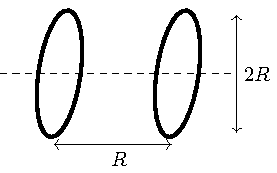
\includegraphics{May2023/3-2.pdf}
\end{center}


}

\sol{

The magnetic field for any localized current distribution $\vec{J}$ is given by
\begin{align}
    \vec{B}(\vec{r}) = \frac{\mu_0}{4 \pi} \int \dd[3]{\vec{r'}} \frac{\vec{J}(\vec{r'}) \cross (\vec{r} - \vec{r}')}{|\vec{r} - \vec{r}'|^3}
\end{align}
Calculating such an integral for any point in space is likely quite difficult, if even possible for the Helmholtz coil setup, so we restrict ourselves to the axis passing through the centers of the coils.
Notice that we can sum the magnetic fields produced by each coil separately, so let us calculate the field produced on this axis (the positive direction is determined by the right hand rule) by a single coil first, where the origin for now is at the center of this coil:
\begin{align}
    \vec{B} = \frac{\mu_0 N I R}{4 \pi} \int_{0}^{2 \pi} \frac{\dd{\phi} \vhat{\phi} \cross (z \vhat{z} - R \vhat{r})}{(R^2 + z^2)^{3/2}} = \frac{\mu_0 N I R^2}{2 (z^2 + R^2)^{3/2}} \vhat{z}
.\end{align}
If we shift our origin to the center of these coils and sum the two contributions, we find
\begin{align}
    \eqbox{ \vec{B} = \frac{\mu_0 N I R^2}{2} \Bigg\{ \frac{1}{[(z + R/2)^2 + R^2]^{3/2}} + \frac{1}{[(z - R/2)^2 + R^2]^{3/2}} \Bigg\} \vhat{z} }
.\end{align}
Notice that for $z \ll R$, the magnetic field
\begin{align}
    \vec{B} = \frac{\mu_0 N I}{2 R} \Bigg[ \underbrace{ \frac{16}{5 \sqrt{5}} }_{1.43} - \underbrace{ \frac{2304}{625 \sqrt{5}} }_{1.65} \Big( \frac{z}{R} \Big)^4 + \hdots \Bigg]
,\end{align}
which suggests that the magnetic field varies only slightly for small deviations from the center of the coils (note: the expansion was performed with Wolfram, so it is likely not expected to be performed by hand on the exam).

}


\prob{3.3}{

The space between the plates of a plane capacitor is filled with two layers 1 and 2 of thicknesses $d_1$ and $d_2$ and permittivities $\epsilon_1$ and $\epsilon_2$, respectively.
Calculate:

\begin{parts}
    \item The capacitance of this capacitor

    \item Charge density at the interface between layers 1 and 2 caused by the voltage $V$ on the capacitor.
\end{parts}

}

\sol{

(a) The relevant equation here is Gauss' law for the electric displacement:
\begin{align}
    \grad \cdot \vec{D} = \rho \longleftrightarrow \oint \dd{\vec{S}} \cdot \vec{D} = Q
,\end{align}
where $\rho$ is the free charge density and $Q$ is the free charged in the volume enclosed by $S$.
Using a Gaussian pillbox, stradling both sides of one metal plate:
\begin{align}
    \vec{D} = \sigma \vhat{n}
,\end{align}
where $\vhat{n}$ is a unit vector pointing from the positively charged plate to the negatively charged plate.
Now we can compute the electric field, assuming that both media are linear:
\begin{align}
    \vec{E} = \frac{\vec{D}}{\epsilon(x)}
,\end{align}
where
\begin{align}
    \epsilon(x) = \begin{cases}
        \epsilon_1 & 0 < x < d_1 \\
        \epsilon_2 & d_1 < x < d_2
    .\end{cases}
\end{align}
From this, we can determine the potential difference between the plates via the following line integral:
\begin{align}
    V = \Bigg| \int_{0}^{d_2} \dd{\vec{r}} \cdot \vec{E} \Bigg| = \sigma \Big( \frac{d_1}{\epsilon_1} + \frac{d_2}{\epsilon_2} \Big)
.\end{align}
And, finally, the capacitance
\begin{align}
    \eqbox{ C = \frac{Q}{V} = A \Big( \frac{d_1}{\epsilon_1} + \frac{d_2}{\epsilon_2} \Big)^{-1} }
.\end{align}
Notice that this reduces to the usual result $C = A \epsilon_0 / d$ when $\epsilon_1 = \epsilon_2 = \epsilon_0$ and $d_1 + d_2 = d$.

(b) The bound surface charge at the interface is
\begin{align}
    \sigma_b = \vec{P} \cdot \vhat{n} = (\epsilon - \epsilon_0) \vec{E} \cdot \vhat{n}
,\end{align}
where we have used $\vec{P} = \chi_e \vec{E}$ and $\chi_e = \epsilon - \epsilon_0$.
Thus, 
\begin{align}
    \eqbox{ \sigma_b = (\epsilon_1 - \epsilon_0) \frac{\sigma}{\epsilon_1} - (\epsilon_2 - \epsilon_0) \frac{\sigma}{\epsilon_2} = \sigma \epsilon_0 \Big( \frac{1}{\epsilon_2} - \frac{1}{\epsilon_1} \Big) }
.\end{align}
Note that the sign depends on the relative polarizability of the dielectrics.

}

\subsection*{Quantum Mechanics}
\addcontentsline{toc}{subsection}{Quantum Mechanics}

\prob{3.4}{

A neutral particle with spin-1/2 and a nonzero magnetic momentum is subject to a periodic magnetic field $B(t) = B_0 \cos{\omega t}$ applied along the $z$-axis.
The state vector of the spin at $t = 0$ is given by:
\begin{align*}
    \bra{\psi(0)} = \begin{pmatrix}
        e^{i \varphi_1} \cos{\theta} & e^{i \varphi_2} \sin{\theta}
    \end{pmatrix}
.\end{align*}
Calculate the expectation values of the spin components $\expval{S_{z}(t)}$, $\expval{S_x(t)}$, and $\expval{S_y(t)}$ at $t > 0$.

}

\sol{

The Hamiltonian for a neutral spin-1/2 particle immersed in a magnetic field is given by
\begin{align}
    H = - \frac{g e}{2 m c} \vec{S} \cdot \vec{B} = -\frac{g e B_0}{2 m c} \cos{\omega t} S_z
,\end{align}
where $g$ is the gyromagnetic factor of the particle.
Observe that our eigenstates are just $\ket{\pm}$, so any arbitrary state
\begin{align}
    \ket{\psi(t)} = c_+(t) \ket{+} + c_-(t) \ket{-}
.\end{align}
We can determine how the coefficients change with time by inserting this expansion into the Schr\"{o}dinger equation:
\begin{align}
    i \hbar \dv{\ket{\psi}}{t} = H \ket{\psi} \Rightarrow \dv{c_{\pm}}{t} = \pm i \alpha \cos{\omega t} \, c_{\pm} \Rightarrow c_{\pm}(t) = c_{\pm}(0) e^{\pm i (\alpha/\omega) \sin(\omega t)}
,\end{align}
where $\alpha = g e B_0/(2 m \hbar c)$.
Thus, the state as a function of time
\begin{align}
    \ket{\psi(t)} = \begin{pmatrix}
        e^{i [ \varphi_1 + (\alpha / \omega) \sin{\omega t} ]} \cos{\theta} \\
        e^{i[ \varphi_2 - (\alpha / \omega) \sin{\omega t} ]} \sin{\theta}
    \end{pmatrix} = e^{i[ \varphi_2 - (\alpha / \omega) \sin{\omega t} ]}  \begin{pmatrix}
        e^{i [ (\varphi_1 - \varphi_2) + 2 (\alpha / \omega) \sin{\omega t} ]} \cos{\theta} \\
        \sin{\theta}
    \end{pmatrix}
.\end{align}
The requested expectation values are then as follows:
\begin{align}
\eqbox{
\begin{aligned}
    \expval{S_x(t)} &=  \frac{\hbar}{2} \cos[(\varphi_1 - \varphi_2) + 2(\alpha / \omega) \sin{\omega t}] \sin(2 \theta) \\
    \expval{S_y(t)} &= -\frac{\hbar}{2} \sin[(\varphi_1 - \varphi_2) + 2(\alpha / \omega) \sin{\omega t}] \sin(2 \theta) \\
    \expval{S_z(t)} &= \frac{\hbar}{2} \cos(2 \theta)
\end{aligned}
}.
\end{align}
Note that the $S_z$ expectation value is independent of time, which is consistent with the Ehrenfest theorem given that $[H,S_z] = 0$ for all $t$.
Also, as a sanity check, we have $\expval{\vec{S}^2} = 3 \hbar^2 / 4$ as expected (again constant in time since $[\vec{S}^2,S_z] = 0$ and therefore that $[\vec{S}^2,H] = 0$.

}


\prob{4.1}{

Assuming that the eigenfunctions for the hydrogen atom are of the form $r^{\beta}e^{-\gamma r} Y_{lm}(\Omega)$ with undetermined parameters $\beta$ and $\gamma$, solve the Schr\"{o}dinger equation.
Are all eigenfunctions and eigenvalues obtained this way?
Justify your answer.

}

\sol{

The Schr\"{o}dinger equation for a central potential reads
\begin{align}
    \Big[ -\frac{\hbar^2}{2 \mu r^2} \pdv{r} r^2 \pdv{r} + \frac{\vec{L}^2}{2 \mu r^2} + V(r)  \Big] \psi(r) = E \psi(r)
.\end{align}
If we put in the solution ansatz, we obtain
\begin{gather}
    -\frac{\hbar^2}{2 \mu} \Big[ \gamma^2 r^{\beta} - 2 \gamma (\beta + 1) r^{\beta - 1} + \beta (\beta + 1) r^{\beta - 2} \Big] + \frac{\hbar^2 l(l+1)}{2 \mu} r^{\beta-2} - e^2 r^{\beta - 1} = E r^{\beta}
.\end{gather}
Equating the coefficients of powers of $r$, we obtain three equations
\begin{align}
\begin{cases}
    E = -\frac{\hbar^2 \gamma^2}{2 \mu} \\
    \gamma (\beta + 1) = \frac{\mu e^2}{\hbar^2} \\
    \beta(\beta + 1) - l(l + 1) = 0
.\end{cases}   
\end{align}
The latter equation has two solutions: $\beta = l,-l-1$, but the first is the only physically admissibly one since for $l > 1$ the second leads to non-normalizable solutions.
We thus choose
\begin{align}
    \eqbox{ \beta = l }
\end{align}
The second equation then yields
\begin{align}
    \eqbox{ \gamma = \frac{\mu e^2}{\hbar^2(l + 1)} }
.\end{align}
Putting this into our first equation above, the energy
\begin{align}
    \eqbox{ E = -\frac{\mu^2 e^2}{\hbar^2 (l + 1)^2} }
.\end{align}
This exactly reproduces the energy levels if we set $n = l + 1$, but our solution ansatz does not capture the full spectrum of the Hydrogen atom, which can be observed by noting that the degeneracy for each energy level implied by the solution above is $2 l + 1$.
The correct degeneracy, though, is $n^2$.

}


\prob{4.2}{

Consider a quantum mechanical system that is described by the Hamiltonian
\begin{align*}
    \hat{H} = \frac{\hat{\vb*{L}}^2}{2I} + a \hat{L}_z + b \hat{L}_z^2
,\end{align*}
where $\hat{\vb*{L}}$ is the angular momentum operator and $I$, $a$, and $b$ are constants.

\begin{parts}
    \item Why do the constants $I$, $a$, and $b$ have to be real-valued parameters?

    \item What are the eigenvalues and eigenstates of $\hat{H}$

    \item Now consider $a = 4 \hbar / I$, $b = 2/I$.
    What is the ground state and the ground state energy of the system?

    \item At time $t = 0$, the system is in the state
    \begin{align*}
        \ket{\psi(t = 0)} = \frac{1}{\sqrt{3}} ( \ket{1,0} + \ket{1,1} - \ket{1,-1} )
    \end{align*}
    Here, we use the usual $\ket{l,m}$ notation to denote the angular momentum eigenstates.
    Determine the time evolution of the state $\ket{\psi(t)}$.
\end{parts}

}

\sol{

(a) Since the Hamiltonian represents a physical observable, it must be Hermitian.
That is,
\begin{align}
    H^{\dagger} = \frac{\vec{L}^2}{2 I^{*}} + a^{*} L_z + b^{*} L_z^2 = \frac{\vec{L}^2}{2 I} + a L_z + b L_z^2
,\end{align}
which can only be true if $I$, $a$, and $b$ are real.

(b) The eigenstates of the Hamiltonian are just those of $\vec{L}^2$ and $L_z$, where
\begin{align}
    \vec{L}^2 \ket{l m} = \hbar^2 l (l + 1)\ket{lm}   , \quad L_z \ket{l m} = \hbar m \ket{lm}    
,\end{align}
$l = 0, 1, \hdots$, and $m = -l , -l-1, \hdots, l-1, l+1$, so
\begin{align}
    \eqbox{ H \ket{lm} = \underbrace{ \Big( \frac{\hbar^2 l (l + 1)}{2 I} + a \hbar m + b \hbar^2 m^2 \Big) }_{E_{lm}} \ket{l m} }
.\end{align}

(c) For the constants given above, the energies read
\begin{align}
    E_{lm} = \frac{\hbar^2 l (l + 1)}{2 I} + \frac{4 \hbar}{I} \hbar m + \frac{2}{I} \hbar^2 m^2 = \frac{\hbar^2}{2 I} \Big( l(l + 1) + 8m + 4m^2 \Big)
.\end{align}
From this, we see that we should minimize with respect to $l$ and $m$:
\begin{align}
    \pdv{E_{lm}}{l} &= 2l + 1 = 0 \Rightarrow l = 1/2 \\
    \pdv{E_{lm}}{m} &= 8 + 8m = 0 \Rightarrow m = -1
.\end{align}
The minimum for $l$ is not physical, but since the $l$ dependence is quadratic, the $l = 0$ and $l = 1$ states give the same contribution.
Our minimum for $m$ requires $l = 1$, so our ground state and ground state energy are
\begin{align}
    \eqbox{ \ket{1, -1} \Leftrightarrow E_{1,-1} = -\frac{\hbar^2}{I} }
.\end{align}


(d) The time evolution is given by
\begin{align}
    \eqbox{ \ket{\psi(t)} = e^{-i H t / \hbar} \ket{\psi(0)} = \frac{1}{\sqrt{3}} \Big( e^{-i \hbar t / I} \ket{1 0} + e^{-7 i \hbar t / I} \ket{1 1} - e^{i \hbar t / I } \ket{1 \, -1} \Big) }
\end{align}

}


\prob{4.3}{

Consider a hydrogen-like atom described by the Hamiltonian
\begin{align*}
    H = \Big( c \sqrt{ \vb*{p}^2 + (mc)^2 } - mc^2 \Big) - \frac{Z e^2}{r}
,\end{align*}
where $m$ is the mass of the electron and $Ze$ is the nuclear charge with $Z \gg 1$.
Since the typical velocity of the electron in such a system is of the order of $Z \alpha c$ (here $\alpha \approx 1/137$ is the fine structure constant and $c$ is the speed of light), it is physically sensible to presenent the electron kinetic energy operator by its relativistic expression.

\begin{parts}
    \item Expand the kinetic energy operator in powers of $[\vb*{p}/(mc)]^2$, and show that the Hamiltonian can be written as
    \begin{align*}
        H = H_0 + V \quad {\rm with}~ H_0 = \frac{\vb*{p}^2}{2m} - \frac{Ze^2}{r}
    ,\end{align*}
    and $V$ is the perturbation consisting of the leading correction to the non-relativistic kinetic energy operator.
    Show that the operator $V$ can be expressed as
    \begin{align*}
        V = -\frac{1}{2mc^2} \Big( H_0 + \frac{Ze^2}{r} \Big)^2
    \end{align*}
    Express your results in terms of $Z$, $\alpha$, and $mc^2$.

    \item Consider the first excited level having $n = 2$, which is four-fold degenerate (spin degrees of freedom are ignored).
    Obtain the first-order corrections to the unperturbed energy $\epsilon_2$, expressing your results in terms of $Z$, $\alpha$, and $mc^2$.
    Does the perturbation lift the degeneracy of this level completely or only partially?
    Would you expect degeneracy to persist in high orders of perturbation theory?
    Justify your answers.
\end{parts}

\textbf{Hints}: The unperturbed bound-state energies are
\begin{align*}
    \epsilon_n = -\frac{(Z\alpha)^2}{2n^2} mc^2 \quad n = 1,2,\cdots~
,\end{align*}
where $\alpha = e^2/(\hbar c)$ is the fine structure constant.
The radial wave functions with $n = 2$ are given by
\begin{align*}
    R_{20}(x) = \frac{1}{\sqrt{2}} \Big( \frac{Z}{a_0} \Big)^{3/2} \Big( 1 - \frac{x}{2} \Big) e^{-x/2}, \quad R_{21}(x) = \frac{1}{2\sqrt{6}} \Big( \frac{Z}{a_0} \Big)^{3/2} x e^{-x/2} 
,\end{align*}
where $x = Zr/a_0$ and $a_0$ is the Bohr radius,
\begin{align*}
    a_0 = \frac{\hbar^2}{m e^2} = \frac{1}{\alpha} \frac{\hbar}{m c} \quad {\rm and} \quad \frac{e^2}{a_0} = \alpha^2 m c^2
.\end{align*}
The following integral may be useful
\begin{align*}
    \int_{0}^{\infty} \dd{x} \, x^n e^{-\gamma x} = \frac{n!}{\gamma^{n+1}}, \quad n \geq 0
.\end{align*}

}

\sol{

(a) We rewrite the Hamiltonian as requested:
\begin{align}
    H &=  mc^2 \Big( \sqrt{1 + [\vec{p}/(mc)]^2} - 1 \Big) - \frac{Z e^2}{r} = mc^2 \Big( \frac{\vec{p}^2}{2 (mc)^2} - \frac{\vec{p}^4}{8(mc)^4} + \hdots \Big) - \frac{Z e^2}{r} \nonumber \\
    &= \eqbox{ \underbrace{ \frac{\vec{p}^2}{2 m} - \frac{Z e^2}{r} }_{H_0} \underbrace{ - \frac{\vec{p}^4}{8 m^3 c^2} }_{V} }
.\end{align}
Observe that we can write
\begin{align}
    \vec{p}^2 = 2m \Big( H_0 + \frac{Z e^2}{r} \Big)
,\end{align}
allowing us to express
\begin{align}
    \eqbox{ V = -\frac{1}{8 m^3 c^2} \Bigg[ 2m \Big( H_0 + \frac{Z e^2}{r} \Big) \Bigg]^2 = -\frac{1}{2 m c^2} \Big( H_0 + \frac{Z e^2}{r} \Big)^2 }
.\end{align}

(b) We must diagonalize the perturbation with respect to the degenerate $n = 2$ states.
Consider the generic matrix element
\begin{align}
    \mel{\phi_{2lm}}{V}{\phi_{2l'm'}} &= -\frac{1}{2mc^2} \mel{\phi_{2lm}}{\Big[ H_0^2 + H_0 \frac{Ze^2}{r} + \frac{Ze^2}{r} H_0 + \frac{Z^2 e^4}{r^2} \Big]}{\phi_{2l'm'}} \nonumber \\
    &= -\frac{1}{2 m c^2} \Big[ \epsilon_2^2 \delta_{l l'} \delta_{m m'} + Z e^2 \epsilon_2 \mel{\phi_{2lm}}{\frac{1}{r}}{\phi_{2l'm'}} + Z^2 e^4 \mel{\phi_{2lm}}{\frac{1}{r^2}}{\phi_{2l'm'}} \Big]
.\end{align}
We must determine the matrix elements
\begin{align}
    \mel{\phi_{2lm}}{\frac{1}{r^k}}{\phi_{2l'm'}} &= \int \dd[3]{\vec{r}} \frac{1}{r^k} R_{2l}(r) Y_{lm}(\Omega) R_{2l'}(r) Y_{l'm'}(\Omega) \nonumber \\
    &= \delta_{l l'} \delta_{m m'} \int_{0}^{\infty} \dd{r} r^{2-k} R_{2l}^{2}(r) = \delta_{l l'} \delta_{m m'} \underbrace{ \Big( \frac{a_0}{Z} \Big)^{3-k} \int_{0}^{\infty} \dd{x} x^{2-k} R_{2l}^{2}(x) }_{I_{lk}}
.\end{align}
Observe that the integral is independent of $m$, so we only have the four integrals as follows:
\begin{align}
    I_{01} &= \frac{Z}{2 a_0} \int_{0}^{\infty} \dd{x} x \Big( 1 - \frac{x}{2} \Big)^2 e^{-x} = \frac{Z}{2 a_0} \int_{0}^{\infty} \dd{x} \Big( x - x^2 + \frac{x^3}{4} \Big) e^{-x} = \frac{Z}{4 a_0} \\
%
    I_{02} &= \frac{Z^2}{2 a_0^2} \int_{0}^{\infty} \dd{x} \Big( 1 - x + \frac{x^2}{4} \Big) e^{-x} = \frac{Z^2}{4 a_0^2} \\
%
    I_{11} &= \frac{Z}{24 a_0} \int_{0}^{\infty} \dd{x} x^3 e^{-x} = \frac{Z}{4 a_0} \\
    I_{12} &= \frac{Z^2}{24 a_0^2} \int_{0}^{\infty} \dd{x} x^2 e^{-x} = \frac{Z^2}{12 a_0^2}
\end{align}
The matrix elements are diagonal in $l$ and $m$, and those elements are independent of $m$.
Thus,
\begin{align}
\eqbox{
\begin{aligned}
    \epsilon_{20}^{(1)} &= -\frac{19 \epsilon_2^2}{2 m c^2} \\
    \epsilon_{21}^{(1)} &= -\frac{25 \epsilon_2^2}{6 m c^2}
\end{aligned}
}
.\end{align}


}


\prob{4.4}{

Consider a particle of charge $q$ (take $q$ to be positive) in a magnetic field $\vb*{B}(\vb*{r})$.
The velocity operator is given by
\begin{align*}
    \vb*{v} = \frac{1}{m} \Big[ -i\hbar \vb*{\nabla} - \frac{q}{c} \vb*{A}(\vb*{r}) \Big], \quad \vb*{B}(\vb*{r}) = \vb*{\nabla} \times \vb*{A}(\vb*{r})
,\end{align*}
where $\vb*{A}(\vb*{r})$ is the vector potential.
Show that
\begin{align*}
    [v_i,v_j] = i \frac{q \hbar}{m^2 c} \epsilon_{ijk} B_k(\vb*{r})
.\end{align*}
Suppose the particle is constrained to move in the $xy$-plane under the influence of a uniform magnetic field directed along the $\hat{\vb*{z}}$-axis.
The Hamiltonian is given by
\begin{align*}
    H = \frac{m}{2} ( v_x^2 + v_y^2 )
.\end{align*}

\begin{parts}
    \item Define the operators
    \begin{align*}
        \hat{a} = \frac{\alpha}{\sqrt{2}} (v_x + i v_y), \quad \hat{a}^{\dagger} = \frac{\alpha}{\sqrt{2}} (v_x - iv_y)
    \end{align*}
    and determine $\alpha$ such that $[\hat{a},\hat{a}^{\dagger}] = 1$.
    Write the Hamiltonian in terms of $\hat{a}$ and $\hat{a}^{\dagger}$.

    \item Obtain the eigenvalues and eigenstates of the Hamiltonian.
    Are the eigenvalues degenerate?
    Justify your answer.
\end{parts}

}

\sol{

Recall that $[\vec{p},f(\vec{r})]g(\vec{r}) = g(\vec{r}) [\vec{p} f(\vec{r})]$.
Thus,
\begin{align}
    [v_i,v_j] &= \frac{1}{m^2} \Bigg\{ [p_i,p_j] - \frac{q}{c} [p_i,A_j] - \frac{q}{c} [A_i,p_j] + \frac{q^2}{c^2} [A_i,A_j] \Bigg\} \nonumber \\
    &= -\frac{q}{m^2 c} \Bigg[ p_i A_j - p_j A_i \Bigg] = i \frac{q \hbar}{m^2 c} \epsilon_{ijk} (\grad \cross \vec{A})_k = \eqbox{ i \frac{q \hbar}{m^2 c} \epsilon_{ijk} B_k }
.\end{align}

(a) The commutator
\begin{align}
    [a,a^{\dagger}] &= \frac{\alpha^2}{2} \Bigg\{ [v_x,v_x] - i [v_x,v_y] + i [v_y,v_x] + [v_y,v_y] \Bigg\} = \alpha^2 \frac{q \hbar B_z}{m^2 c} = 1 \nonumber \\
    &\Rightarrow \eqbox{ \alpha = \sqrt{\frac{m^2 c}{q \hbar B_z}} }
.\end{align}
Next, we can rearrange the definitions of $a$ and $a^{\dagger}$ to obtain
\begin{align}
    v_x = \frac{1}{\sqrt{2} \alpha} (a + a^{\dagger}), \quad v_x = \frac{1}{\sqrt{2} i \alpha} (a - a^{\dagger})
.\end{align}
Putting this into the Hamiltonian, we find
\begin{align}
    \eqbox{ H = \frac{m}{4 \alpha^2} \Big(a^{\dagger} a + a a^{\dagger} \Big) = \hbar \frac{q B_z}{2 m^3 c} \Big( a^{\dagger} a + \frac{1}{2} \Big) }
.\end{align}

(c) Since $a^{\dagger} a$ is a number operator, we know immediately how to write the spectrum of the Hamiltonian:
\begin{align}
    \eqbox{ H \ket{n} = \hbar \frac{q B_z}{2 m c} (n + 1/2) }
,\end{align}
where $\ket{n}$ satisfies the eigenequation $a^{\dagger}a \ket{n} = n \ket{n}$.

}
